

\chapter{Historical Ciphers}
    \section{Substitution Ciphers}
        \begin{center}
            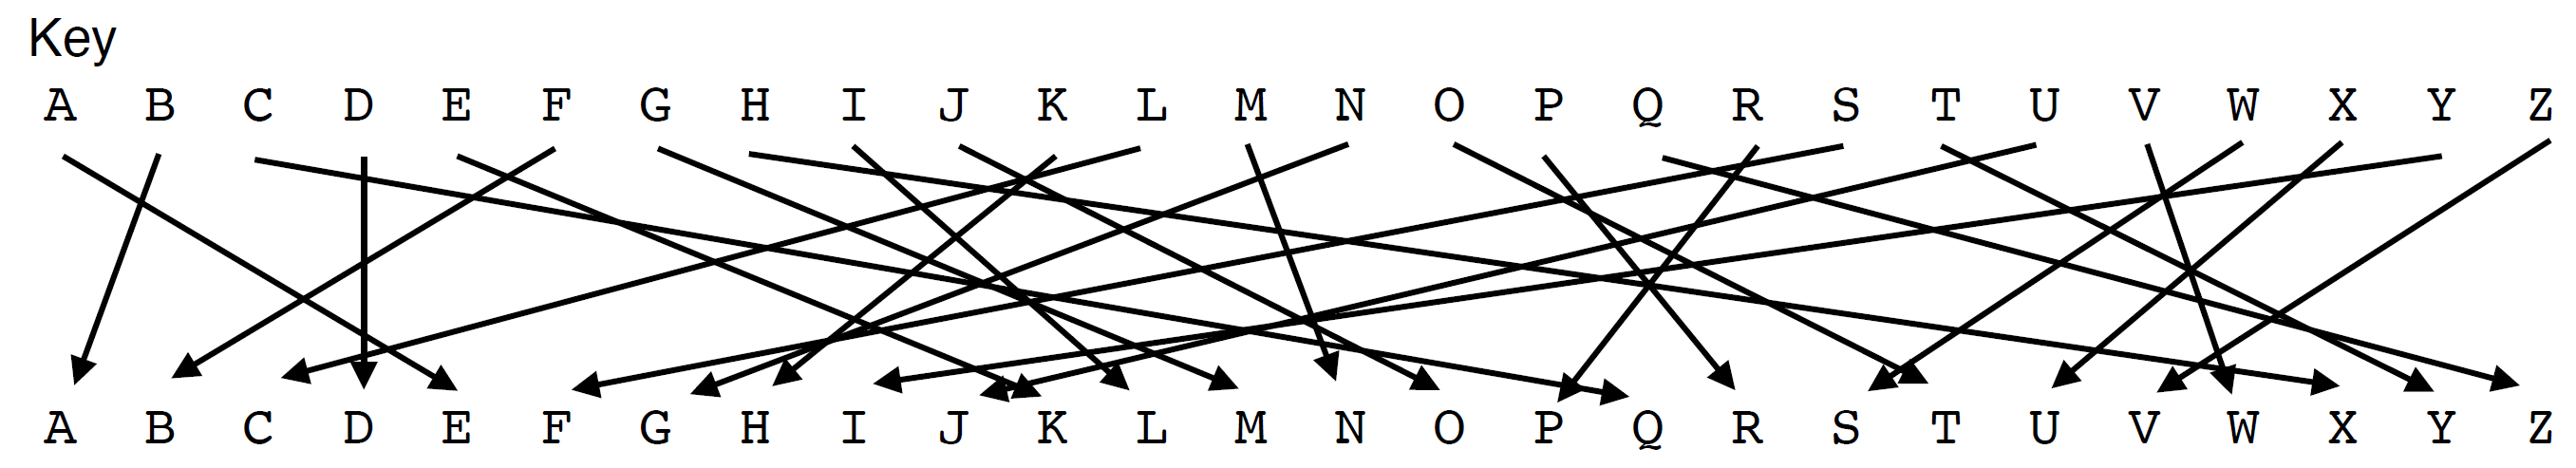
\includegraphics[width=160mm]{Graphics/Historical Ciphers/SubstitutionCiphers1.png}\newline
        \end{center}
        \begin{center}
            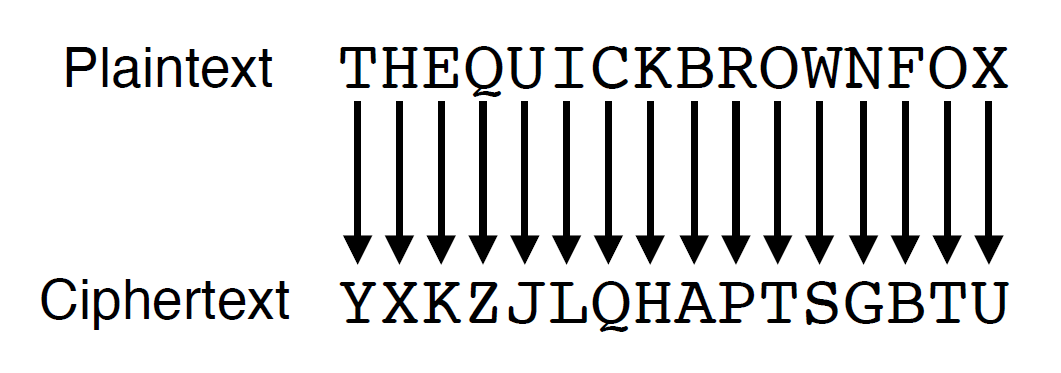
\includegraphics[width=80mm]{Graphics/Historical Ciphers/SubstitutionCiphers2.png}\newline
        \end{center}
        \begin{itemize}
            \item One of the oldest cipher in the world, used in the bible (Atbash)
            \item $\#Keys = 26! \gg 2^{86}$
        \end{itemize}
    
    \section{Caesar Cipher}
        \begin{itemize}
            \item Key is a fixed substitution table which shifts every letter by 3
            \item Encryption and decryption are as in the substitution cipher
        \end{itemize}
        \textbf{Shift Cipher}
        \begin{itemize}
            \item Generalization of Ceasar's Cipher: Variable Shift
            \item $\#Keys = 26$
        \end{itemize}
     
    \section{Vigènere Cipher}
    	\begin{itemize}
    		\item Variant of Caesar/Shift Cipher
    		\item Polyalphabetic Cipher: Not same shift for every plaintext character
    		\item $\# Keys = 26^n$
    	\end{itemize}
    	\begin{center}
          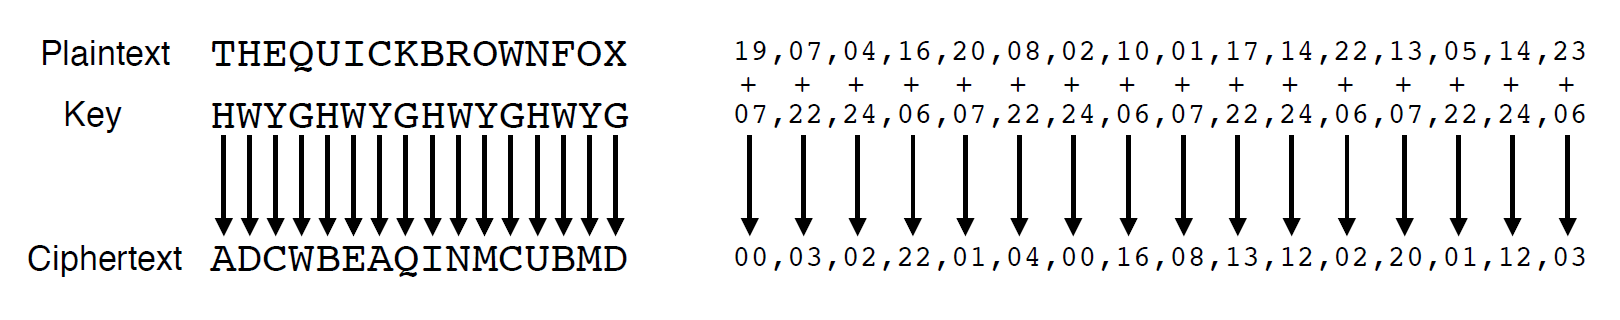
\includegraphics[width=140mm]{Graphics/Historical Ciphers/VigenereCipher.png}\newline
       \end{center}
	
	\section{Cryptanalysis}
		\begin{itemize}
			\item Scytale: Curvature of leather belt is give away
			\item Caesar Scheme: No key! Insecure once the method of encryption is known
			\item Shift Cipher: Key-space too small! Try all 26 keys
			\item What about the substitution and Vigènere ciphers?
		\end{itemize}
		
	\section{Frequency Analysis}
		\begin{itemize}
			\item Idea: Short piece of English text has similar statistics as English language as a whole
			\item Count letter frequencies in natural language
			\item Used for Vigènere Ciphers
		\end{itemize}
    	\begin{center}
         	 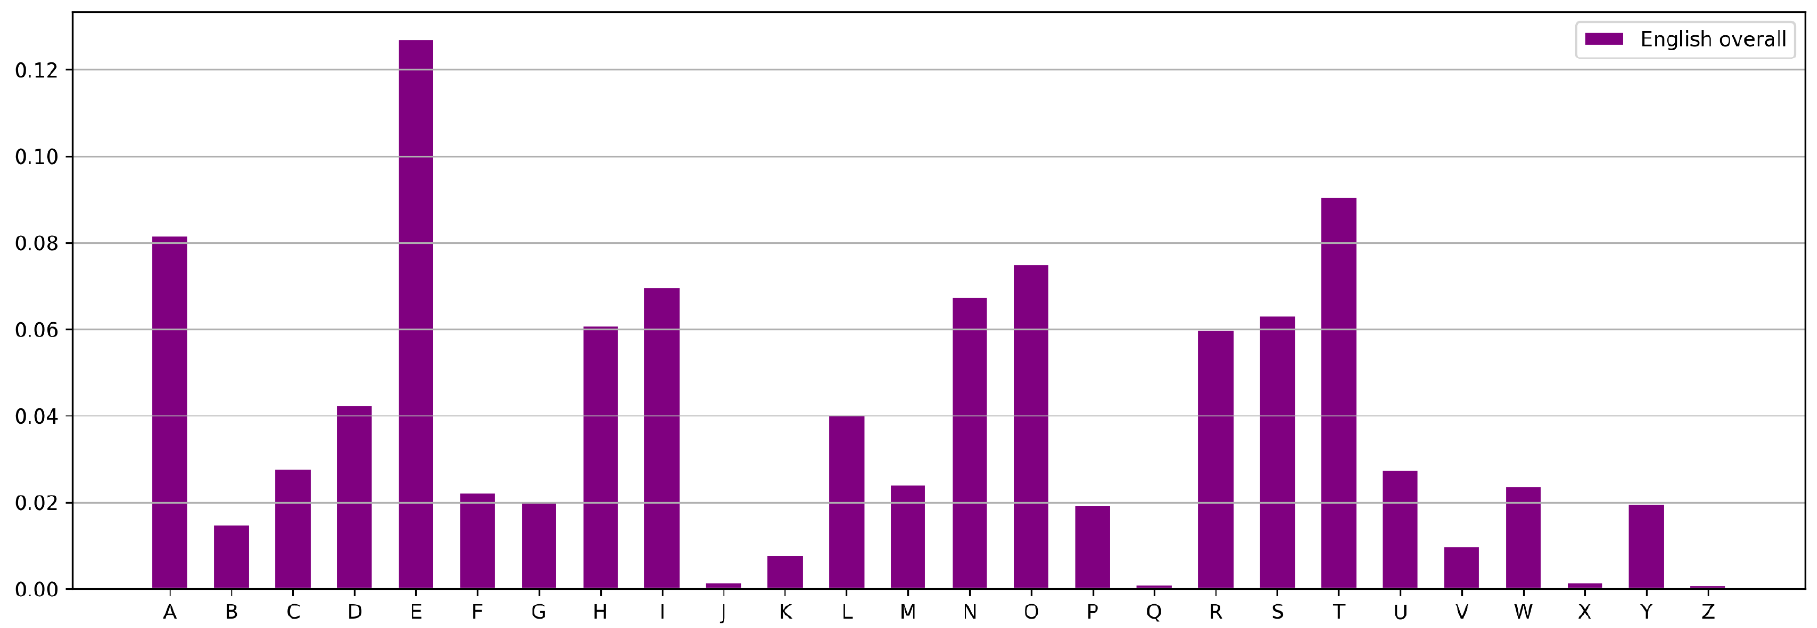
\includegraphics[width=180mm]{Graphics/Historical Ciphers/FrequencyAnalysis.png}\newline
       \end{center}
	
	\section{Cryptanalysis of the Substitution Cipher}
		\begin{itemize}
			\item Natural language also has frequent character constellations
			\item Generalize character frequencies: Bigrams, trigrams … N-grams
			\item Plaintext recovery requires a lot of context information and guessing
		\end{itemize}
		\begin{center}
         	 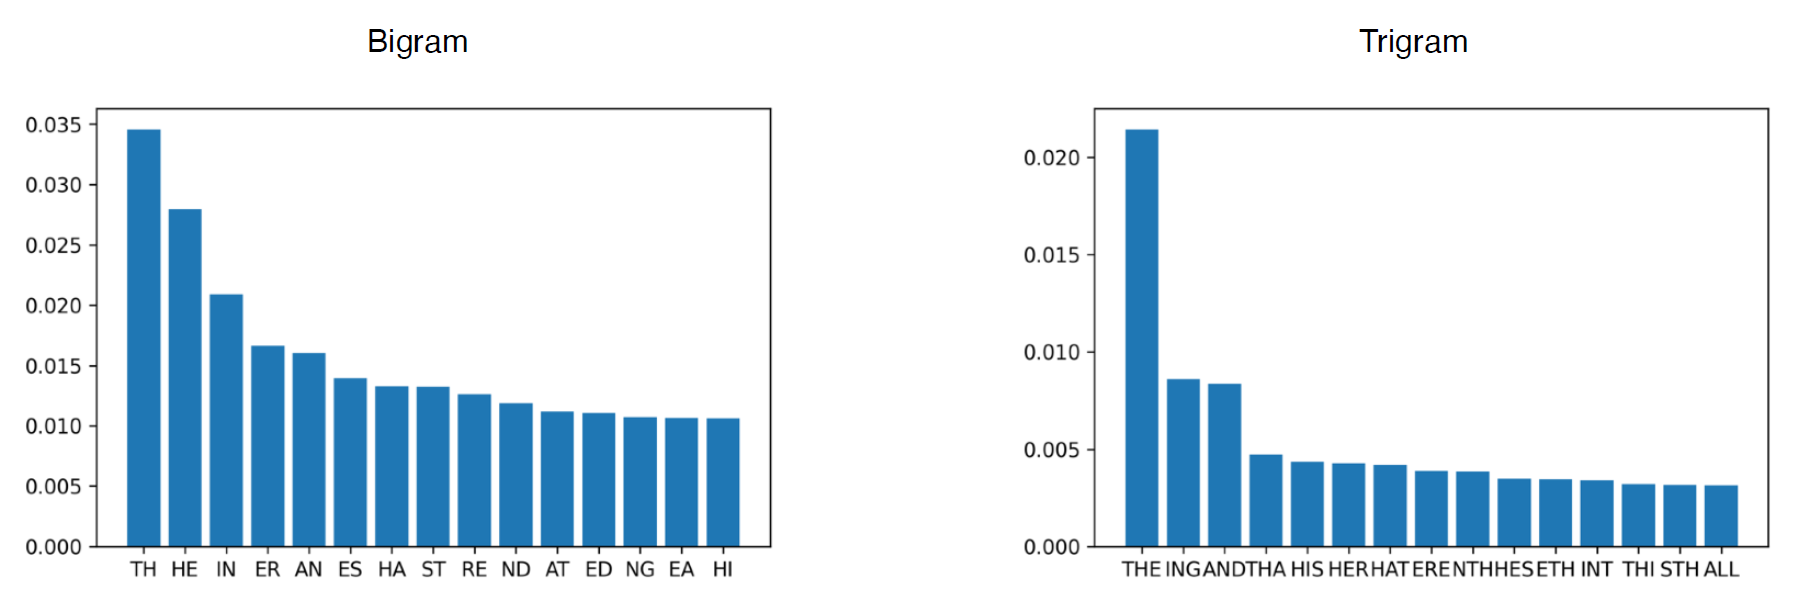
\includegraphics[width=160mm]{Graphics/Historical Ciphers/CryptanalysisSubstitutionCipher1.png}
       \end{center}
       \begin{itemize}
       	\item Plaintext recovery is strongest possible attack
       	\item Requires context information
       	\item More prior knowledge?
       	\item Maximum context information: Ciphertext encrypts one of two messages
       	\item Structural Property of Cipher: Same letters always encrypt to same letter
       \end{itemize}
       \begin{center}
         	 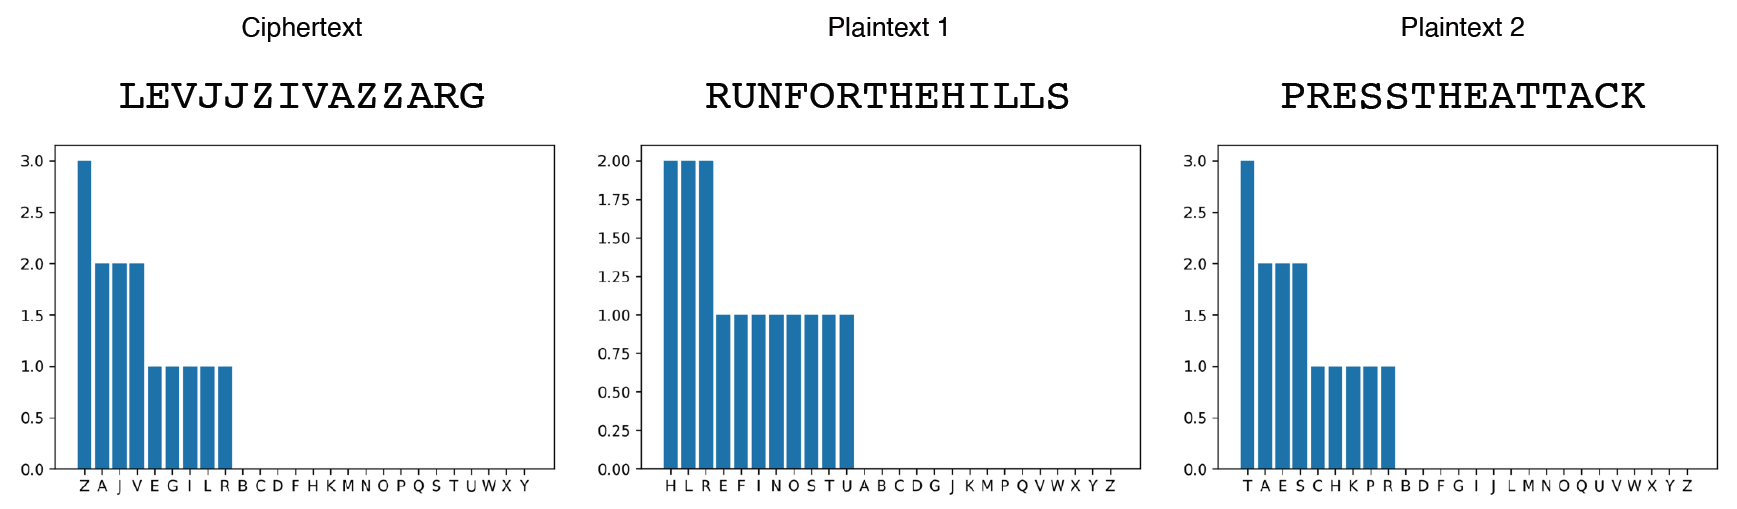
\includegraphics[width=160mm]{Graphics/Historical Ciphers/CryptanalysisSubstitutionCipher2.png}\newline
       \end{center}
    
    \section{Summary}
    	\begin{itemize}
    		\item Historical Ciphers were based on simple character substitution patterns
    		\item Typically small keys spaces
    		\item Can be broken with simple statistical analysis
    		\item Security relied mostly on the fact the method of encryption was not known to the adversary
    	\end{itemize}
    
    \section{Enigma}
    	\begin{itemize}
    		\item Enigma was a family of cipher machines used before and during WWII
    		\item Several of those were used by German forces during WWII
    		\item Cryptanalysis of these machines focused huge Allies effort
    		\item In particular, Turing and Blechtley park
    	\end{itemize}
    	
    	\subsection{General Architecture of Enigma}
    		\begin{itemize}
    			\item Rotor machine with input keyboard and output device
    			\item Includes several layers of transformations to perform encryption
    			\item Encryption is performed letter by letter
    			\item The transformations evolve with time to prevent direct frequency analysis
    			\item The cipher was an involution
    		\end{itemize}
    	
    	\subsection{Basic principle}
    		\begin{itemize}
    			\item Mix of mechanical and electrical technology
    			\item With the light output display : electric circuit from keyboard to lights
    			\item Goes through several stages into and out of the machine
    			\item Mechanical evolution after every key is released
    		\end{itemize}
    		\begin{center}
         	 	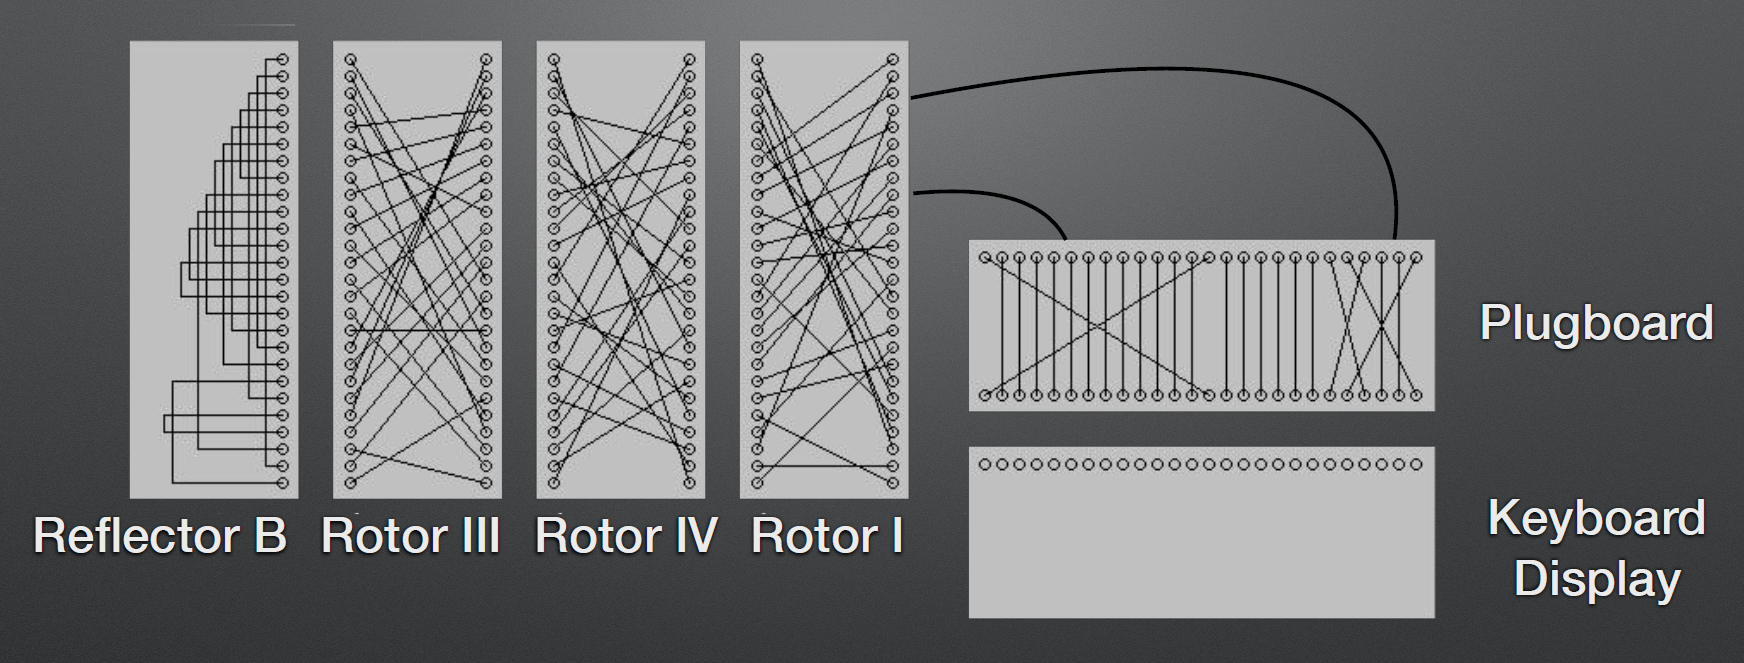
\includegraphics[width=180mm]{Graphics/Historical Ciphers/Enigma.png}\newline
       		\end{center}
       
       	\subsection{Key Size}
       		\begin{itemize}
       			\item Per message key:
       				\begin{itemize}
       					\item 17.576 possibilities (with 3 rotors) $\approx$ 14 bits
       					\item 456.976 possibilities (with 4 rotors) $\approx$ 19 bits
       				\end{itemize}
       			\item Daily key (4 rotor case)$\approx$ 78 bits:
       				\begin{itemize}
       					\item 2 choices of reflector
       					\item 2 choices of fourth rotor
       					\item 336 choices of first three rotors (in set of 8)
       					\item Ring setting : 456.976 possibilities
       					\item Arbitrary plugboard pairing (up to 13 plugs):
       					532.985.208.200.576 possibilities
       				\end{itemize}
       		\end{itemize}
       		Note: There is a dependency between daily and message key\\
       		Total key size $\approx$ 87.5 bits
       	
		\subsection{Digital rewriting of Enigma}
			\begin{itemize}
				\item View the encryption as a sequence of (evolving) permutations on letters
				\begin{itemize}
					\item Step 1: Swap letters according to plugboard
					\item Step 2, 3, 4, (5): Apply permutations corresponding to each rotor in order
					\item Mid Step: Apply (involutive) permutation of the reflector
					\item Step (-5), -4, -3, -2 : Apply inverse rotor permutations
					\item Step -1: Swap letters according to plugboard
				\end{itemize}
				\item Evolve Rotors state
			\end{itemize}

		\subsection{Reflector Permutations}
			\begin{center}
         		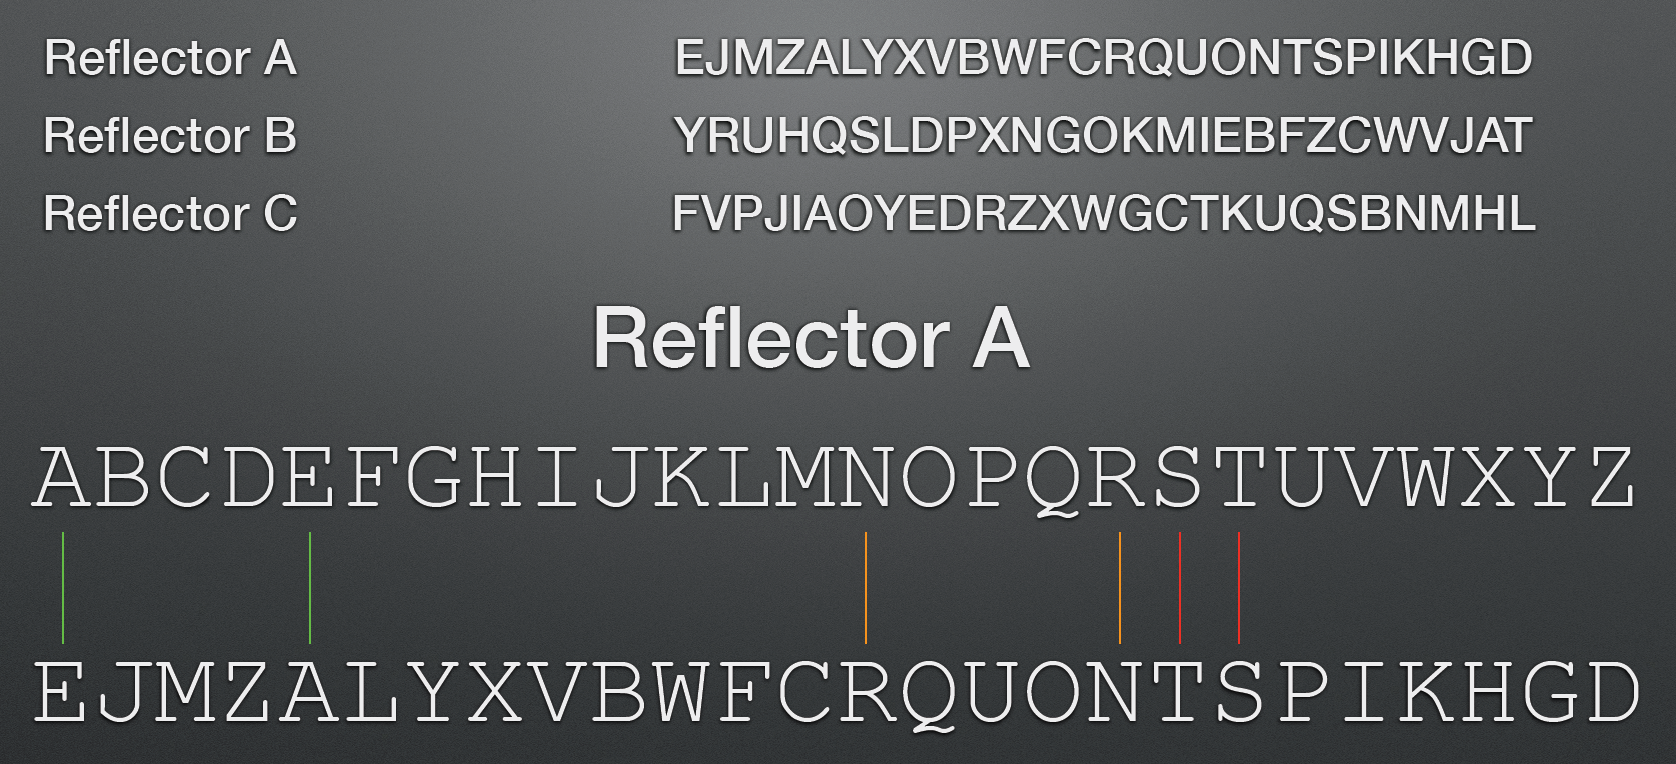
\includegraphics[width=180mm]{Graphics/Historical Ciphers/Enigma2.png}\newline
       		\end{center}
       	
       	\subsection{Rotor Permutations}
       		\begin{center}
         		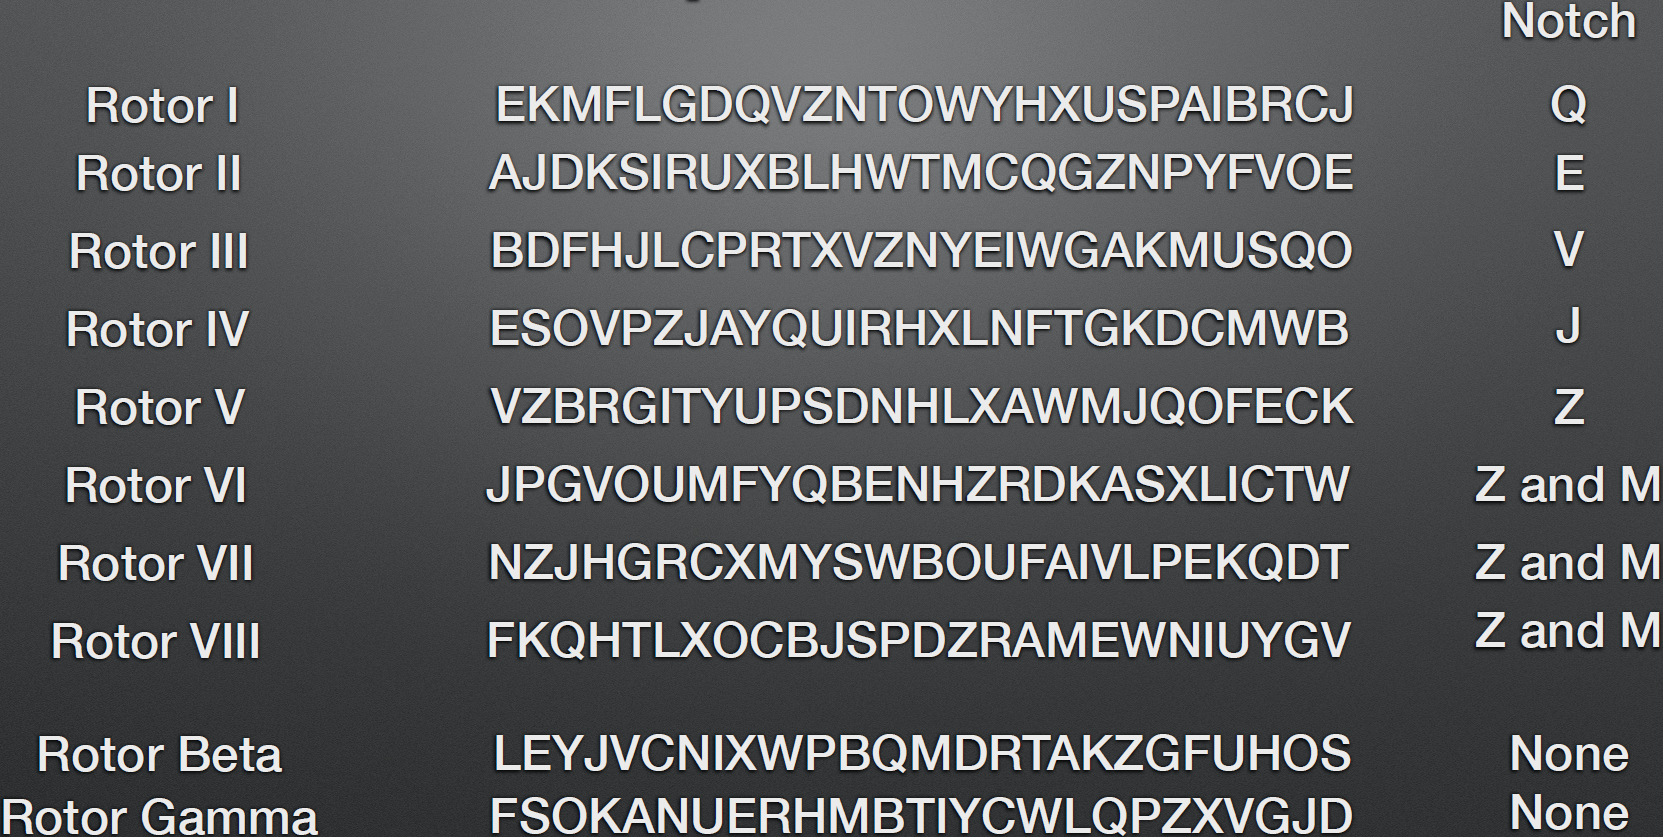
\includegraphics[width=180mm]{Graphics/Historical Ciphers/Enigma3.png}\newline
       		\end{center}
       		\begin{center}
         		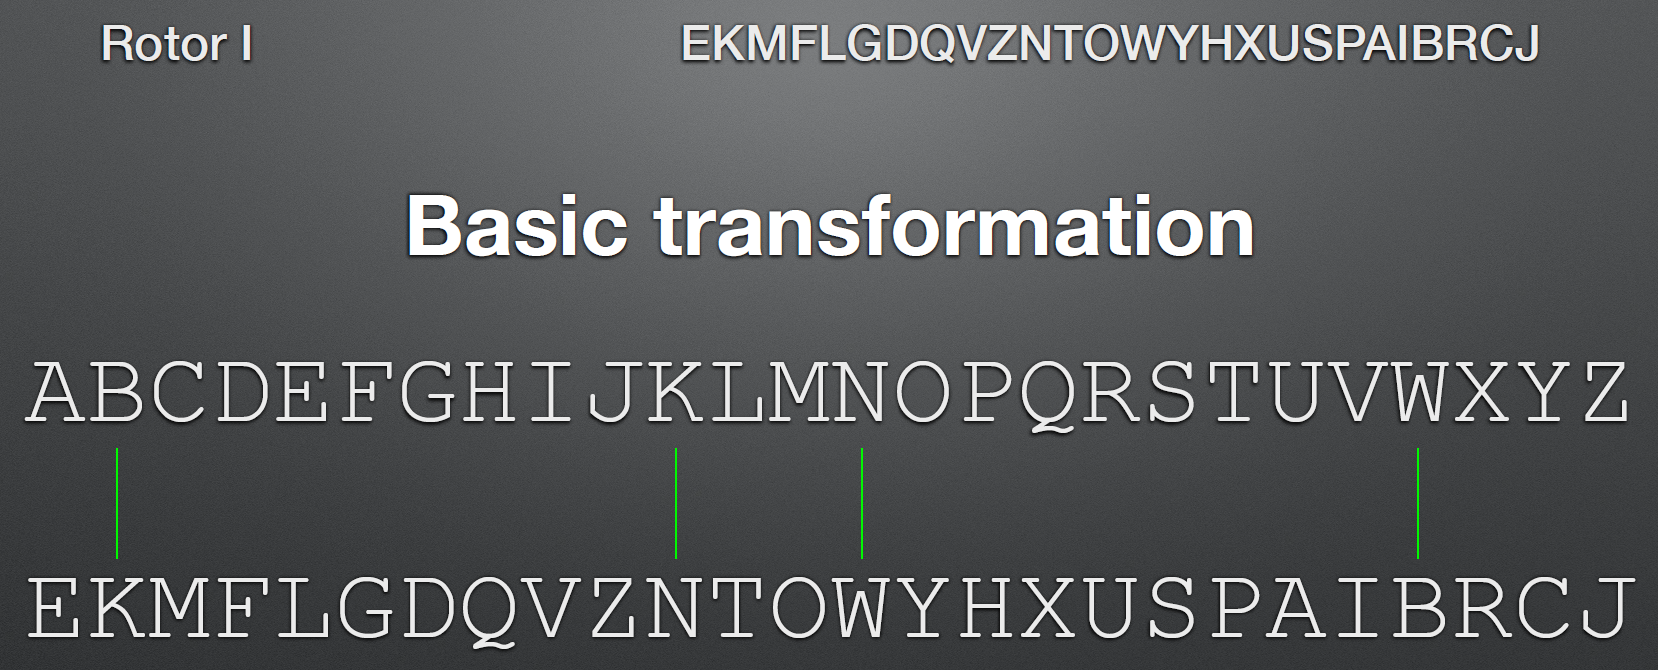
\includegraphics[width=180mm]{Graphics/Historical Ciphers/Enigma4.png}\newline
       		\end{center}
       	
       	\subsection{Rotor permutations (after rotation)}
       		\begin{center}
         		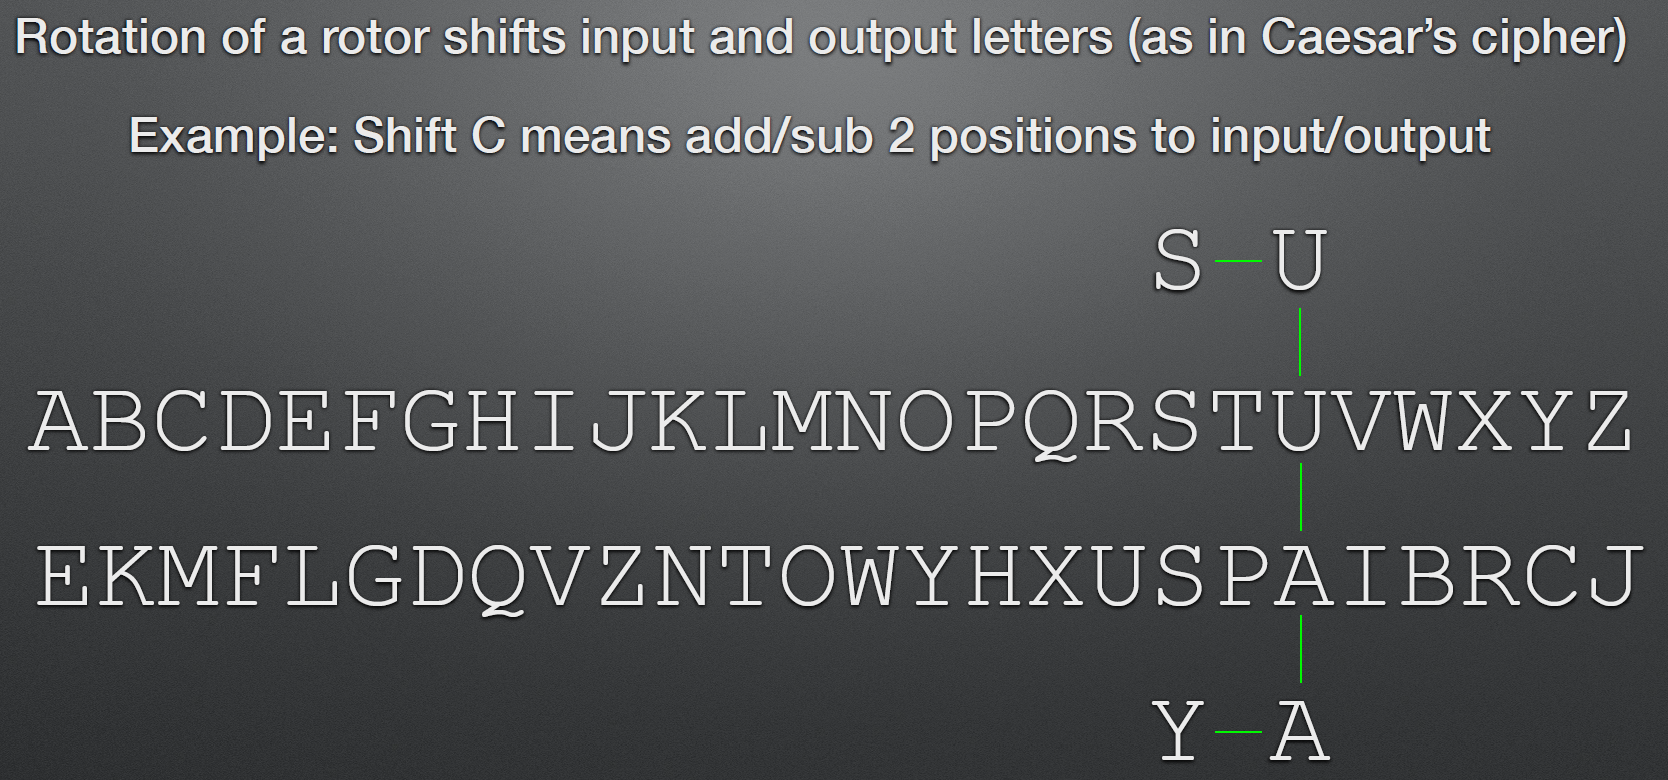
\includegraphics[width=180mm]{Graphics/Historical Ciphers/Enigma5.png}\newline
       		\end{center}
       	
       	\subsection{Plugboard}
       		\begin{center}
         		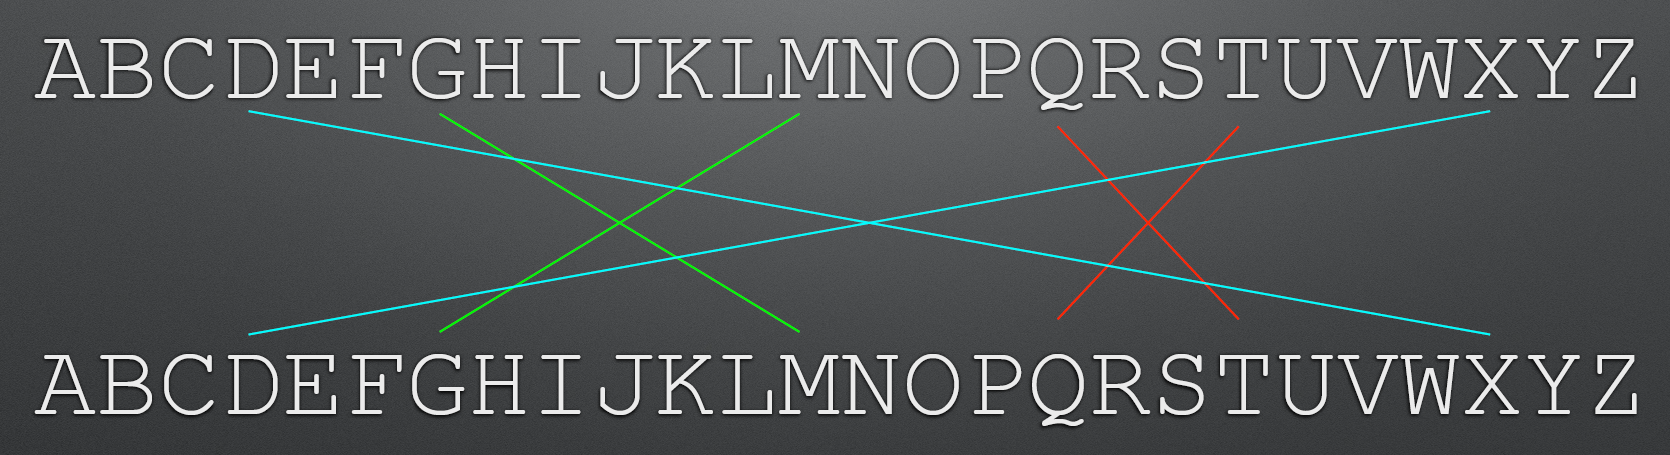
\includegraphics[width=180mm]{Graphics/Historical Ciphers/Enigma6.png}\newline
       		\end{center}
       	
       	\subsection{Rotor Evolution}
       		\begin{itemize}
       			\item Basic evolution: After every key release, rotate right rotor by 1 letter
       				\begin{itemize}
       					\item State A goes to B, B to C, … Y to Z and Z to A
       				\end{itemize}
       			\item Second rotor: If right rotor in notch pos. before change, rotate second rotor
       			\item Third rotor: If second rotor in notch pos., rotate third AND second rotors
       			\item Fourth rotor (optional): Never rotates
       		\end{itemize}
       	
       	\subsection{A simple property of Enigma}
       		\begin{itemize}
       			\item At every time t, the current transformation is an involution with no fixed point
       			\item Proof:
       				\begin{itemize}
       					\item By inspection, this is true for reflectors.
       					\item Let $\pi$ denote the reflector permutation and $\sigma$ be the current permutation of rotors/plugboard.
       					Then, the global permutation is $\sigma^{-1} \circ \pi \circ \sigma$.
       					\item It is an involution since
       					$(\sigma^{-1} \circ \pi \circ \sigma) \circ (\sigma^{-1} \circ \pi \circ \sigma) = \sigma^{-1} \circ \pi \circ \pi \circ \sigma = \sigma^{-1} \circ \sigma = Id$.
       					\item No fixed point since $\sigma^{-1} \circ \pi \circ \sigma(X) = X \implies \pi \circ \sigma(X) = \sigma(X)$\\
       					(impossible for $\pi$).
       				\end{itemize}
       		\end{itemize}
       	
       	\subsection{Modern view on Enigma}
       		\begin{itemize}
       			\item Trivially broken with modern standards
       			\item Example attack 1 (Chosen plaintext distinguisher):\\
       			Encrypt AAA….AAA (100 letters): 
       			Enigma encryption never contains A while random string of the same length has A with prob > 98%
       			\item Example attack 2 : The message is malleable letter by letter
       			\item Example attack 3 (Chosen plaintext attack): 
       			To decrypt challenge cipher text, simply feed it as plaintext to an encryption blackbox. 
       			Because of the involution property, get original plaintext back.
       			\item A simple key recovery faster than exhaustive search
       			\item Important : The cipher has a fixed part and a time varying part.\\
       			More precisely at time $t$ it can be written as $F^{-1} \circ V_t \circ F$.
       			\begin{itemize}
       				\item The fixed part comprised the plugboard and the initial position of first rotor.
       				\item The varying part is the rotors, reflectors and varies with rotations.
       			\end{itemize}
       			\item Key size for $F$ is 26 x 532.985.208.200.576 possibilities $\approx$ 53.6 bits.
       			\item Key size for $V_t$ is 2 x 2 x 336 x 265 possibilities $\approx$ 33.9 bits.
       		\end{itemize}
       	
       	\subsection{Recovering $V_t$ by "cheap" brute force}
       		\begin{itemize}
       			\item We can "fingerprint" $V_t$ with no information on $F$
       			\item Encrypt AAAAA...AAAAAA to $L_1L_2...L_n$ where $L_i = F^{-1} \circ V_i \circ F(A)$
       			\item Note that $L_i = L_j \Leftrightarrow V_i(X)=V_j(X)$ where $X = F(A)$
       			\item Enumerate $X$ and the key of the sequence $V_t$.
       			\item Cost $\approx$ 38.6 bits (with 4 rotos) - At first glance, $+ log_2(n)$ but avoidable
       		\end{itemize}
       	
       	\subsection{Practical Version}
       		\begin{itemize}
       			\item Data collection: Encrypt a sequence of 46 consecutive A — discard first 3
       			\item Fingerprint the 43 letters truncated encrypted sequence as follows:
       				\begin{itemize}
       					\item To each of the last 12 letters:
       						\begin{itemize}
       							\item Associate the position of the first letter in the first 31 that matches it
       							\item If no match, associate the value 0
       						\end{itemize}
       					\item This fingerprint has 60 bits and doesn’t depend on $F$ (except for $F(A)$)
       					\item Enough to identify the varying part $V$ (almost) uniquely
       					\item Once $V$ is obtained, recovering F fully is easy
       				\end{itemize}
       		\end{itemize}

































